\documentclass[12pt,twoside,a4paper]{article}

\textwidth 17cm \textheight 25cm \evensidemargin 0cm
\oddsidemargin 0cm \topmargin -2cm
\parindent 0pt
%\parskip \bigskipamount

\usepackage{graphicx}
\usepackage[dutch]{babel}
\usepackage{amssymb,amsthm,amsmath}
%\usepackage{dot2texi}
\usepackage[utf8]{inputenc}
\usepackage{nopageno}
\usepackage{pdfpages}
\usepackage{enumerate}
\usepackage{caption}
\usepackage{wrapfig}
\usepackage{pgf,tikz,pgfplots}
\pgfplotsset{compat=1.15}
\usepackage{color}
\usetikzlibrary{arrows}
\usetikzlibrary{patterns}
\usepackage{fancyhdr}
\pagestyle{fancy}
\usepackage[version=3]{mhchem}
\usepackage{multicol}
\usepackage{fix-cm}
\usepackage{setspace}
\usepackage{mhchem}
\usepackage{xhfill}
\usepackage{parskip}
\usepackage{cancel}
\usepackage{mdframed}
\usepackage{url}
\usepackage{mathtools}
\usepackage{changepage}

\newcommand{\todo}[1]{{\color{red} TODO: #1}}

\newcommand{\degree}{\ensuremath{^\circ}}
\newcommand\rad{\qopname\relax o{\mathrm{rad}}}

\newcommand\ggd{\qopname\relax o{\mathrm{ggd}}}

\pgfmathdeclarefunction{gauss}{2}{%
  \pgfmathparse{1/(#2*sqrt(2*pi))*exp(-((x-#1)^2)/(2*#2^2))}%
}

\def\LRA{\Leftrightarrow}

\newcommand{\zrmbox}{\framebox{\phantom{EXE}}\phantom{X}}
\newcommand{\zrm}[1]{\framebox{#1}}

% environment oefening:
% houdt een teller bij die de oefeningen nummert, probeert ook de oefening op één pagina te houden
\newcounter{noefening}
\setcounter{noefening}{0}
\newenvironment{oefening}
{
  \stepcounter{noefening}
  \pagebreak[0]
  \begin{minipage}{\textwidth}
  \vspace*{0.7cm}{\large\bf Oefening \arabic{noefening}}
}{%
  \end{minipage}
}

\usepackage{calc}

% vraag
\reversemarginpar
\newcounter{punten}
\setcounter{punten}{0}
\newcounter{nvraag}
\setcounter{nvraag}{1}
\newlength{\puntwidth}
\newlength{\boxwidth}
\newcommand{\vraag}[1]{
\settowidth{\puntwidth}{\Large{#1}}
\setlength{\boxwidth}{1.5cm}
\addtolength{\boxwidth}{-\puntwidth}
{\large\bf Vraag \arabic{nvraag} \addtocounter{nvraag}{1}}\vspace*{-0.5cm}
{\marginpar{\color{lightgray}\fbox{\parbox{1.5cm}{\vspace*{1cm}\hspace*{\boxwidth}{\Large{#1}}}}}
\vspace*{0.5cm}}
\addtocounter{punten}{#1}}

% arulefill
\def\arulefill{\leavevmode{\xrfill[-5pt]{0.3pt}[lightgray]\endgraf}\vspace*{0.2cm}}

% \arules{n}
\newcommand{\arules}[1]{
\color{lightgray}
%\vspace*{0.05cm}
\foreach \n in {1,...,#1}{
  \vspace*{0.75cm}
  \hrule height 0.3pt\hfill
}\color{black}\vspace*{0.2cm}}

% \arule{x}
\newcommand{\arule}[1]{
\color{lightgray}{\raisebox{-0.1cm}{\rule[-0.05cm]{#1}{0.3pt}}}\color{black}
}

% \abox{y}
\newcommand{\abox}[1]{
\fbox{
\begin{minipage}{\textwidth- 4\fboxsep}
\hspace*{\textwidth}\vspace{#1}
\end{minipage}
}
}

\newcommand{\ruitjes}[1]{
\definecolor{cqcqcq}{rgb}{0.85,0.85,0.85}
\hspace*{-2.5cm}
\begin{tikzpicture}[scale=1.04,line cap=round,line join=round,>=triangle 45,x=1.0cm,y=1.0cm]
\draw [color=cqcqcq, xstep=0.5cm, ystep=0.5cm] (0,-#1) grid (20.5,0);
\end{tikzpicture}
}


\newcommand{\assenstelsel}[5][1]{
\definecolor{cqcqcq}{rgb}{0.65,0.65,0.65}
\begin{tikzpicture}[line cap=round,line join=round,>=triangle 45,x=#1cm,y=#1cm]
\draw [color=cqcqcq,dash pattern=on 1pt off 1pt, xstep=1.0cm,ystep=1.0cm] (#2,#4) grid (#3,#5);
\draw[->,color=black] (#2,0) -- (#3,0);
%\draw[shift={(1,0)},color=black] (0pt,2pt) -- (0pt,-2pt) node[below] {\footnotesize $1$};
%\draw[color=black] (#3.25,0.07) node [anchor=south west] {$x$};
\draw[->,color=black] (0,#4) -- (0,#5);
%\draw[shift={(0,1)},color=black] (2pt,0pt) -- (-2pt,0pt) node[left] {\footnotesize $1$};
\draw[color=black] (0.09,#5.25) node [anchor=west] {\phantom{$y$}};
%\draw[color=black] (0pt,-10pt) node[right] {\footnotesize $0$};
\end{tikzpicture}
}

\newcommand{\getallenas}[3][1]{
\definecolor{cqcqcq}{rgb}{0.65,0.65,0.65}
\begin{tikzpicture}[scale=#1,line cap=round,line join=round,>=triangle 45,x=1.0cm,y=1.0cm]
\draw [color=cqcqcq,dash pattern=on 1pt off 1pt, xstep=1.0cm,ystep=1.0cm] (#2,-0.2) grid (#3,0.2);
\draw[->,color=black] (#2.25,0) -- (#3.5,0);
\draw[shift={(0,0)},color=black] (0pt,2pt) -- (0pt,-2pt) node[below] {\footnotesize $0$};
\draw[shift={(1,0)},color=black] (0pt,2pt) -- (0pt,-2pt) node[below] {\footnotesize $1$};
\draw[color=black] (#3.25,0.07) node [anchor=south west] {$\mathbb{R}$};
\end{tikzpicture}
}

\newcommand{\visgraad}[1]{\begin{tabular}{p{0.5cm}|p{#1}}&\\\hline\\\end{tabular}}

\newcommand{\tekenschema}[2]{\begin{tabular}{p{0.5cm}|p{#1}}&\\\hline\\[#2]\end{tabular}}

% schema van Horner
\newcommand{\schemahorner}{
\begin{tabular}{p{0.5cm}|p{7cm}}
&\\[1.5cm]
\hline\\
\end{tabular}}

% geef tabular iets meer ruimte
\setlength{\tabcolsep}{14pt}
\renewcommand{\arraystretch}{1.5}

\newcommand{\toets}[3]{
\thispagestyle{plain}
\vspace*{-2.5cm}
\begin{tikzpicture}[remember picture, overlay]
    \node [shift={(15.25 cm,-1.6cm)}] {%
        \includegraphics[width=1.8cm]{/home/ppareit/kaa1415/logokaavelgem.png}%
    };%
\end{tikzpicture}

\begin{tabular}{|llc|c|}
\hline
\vspace*{-0.5cm}
&&&\\
Naam & \arule{4cm} & {\Large\bf KA AVELGEM} & \\
\vspace*{-0.75cm}
&&&\\
Klas & \arule{4cm} & {\Large\bf 20...-...-...} & \\
\hline
\vspace*{-0.75cm}
&&&\\
Toets & {\bf #2} & {\large\bf #1} & Beoordeling\\
\vspace*{-0.75cm}
&&&\\
Onderwerp & \multicolumn{2}{l|}{\bf #3} &\\
\hline
\end{tabular}
}

\newcommand{\oefeningen}[1]{

\fancyhead[LE, RO]{\vspace{0.5cm} #1}
%\thispagestyle{plain}

{\bf \Large \centering Oefeningen: #1}

}

\raggedbottom

\newcommand\vl{\qopname\relax o{\mathrm{vl}}}

\newcommand\dom{\qopname\relax o{\mathrm{dom}}}
\newcommand\ber{\qopname\relax o{\mathrm{ber}}}

\newcommand\mC{\qopname\relax o{\mathrm{mC}}}
\newcommand\uC{\qopname\relax o{\mathrm{{\mu}C}}}
\newcommand\C{\qopname\relax o{\mathrm{C}}}

\newcommand\W{\qopname\relax o{\mathrm{W}}}
\newcommand\kW{\qopname\relax o{\mathrm{kW}}}
\newcommand\kWh{\qopname\relax o{\mathrm{kWh}}}


\newcommand\V{\qopname\relax o{\mathrm{V}}}
\newcommand\ohm{\qopname\relax o{\mathrm{\Omega}}}
\newcommand\kohm{\qopname\relax o{\mathrm{k\Omega}}}


\newcommand\N{\qopname\relax o{\mathrm{N}}}

\newcommand\Nperkg{\qopname\relax o{\mathrm{N/kg}}}

\newcommand\Nperm{\qopname\relax o{\mathrm{N/m}}}

\newcommand\gpermol{\qopname\relax o{\mathrm{g/mol}}}


\newcommand\kgperm{\qopname\relax o{\mathrm{kg/m}}}
\newcommand\kgperdm{\qopname\relax o{\mathrm{kg/dm}}}
\newcommand\gpercm{\qopname\relax o{\mathrm{g/cm}}}
\newcommand\gperml{\qopname\relax o{\mathrm{g/ml}}}


\newcommand{\mA}{\;\mbox{mA}}
\newcommand{\A}{\;\mbox{A}}
\newcommand{\MA}{\;\mbox{MA}}

\newcommand{\us}{\;\mu\mbox{s}}
\newcommand\s{\qopname\relax o{\mathrm{s}}}

\newcommand\h{\qopname\relax o{\mathrm{h}}}

\newcommand{\kmperh}{\;\mbox{km/h}}
\newcommand{\mpers}{\;\mbox{m/s}}
\newcommand{\kmpermin}{\;\mbox{km/min}}
\newcommand{\kmpers}{\;\mbox{km/s}}

\newcommand{\mph}{\;\mbox{mph}}

\newcommand{\Hz}{\;\mbox{Hz}}

\newcommand\Gm{\qopname\relax o{\mathrm{Gm}}}
\newcommand\Mm{\qopname\relax o{\mathrm{Mm}}}
\newcommand\km{\qopname\relax o{\mathrm{km}}}
\newcommand\hm{\qopname\relax o{\mathrm{hm}}}
\newcommand\dam{\qopname\relax o{\mathrm{dam}}}
\newcommand\m{\qopname\relax o{\mathrm{m}}}
\newcommand\dm{\qopname\relax o{\mathrm{dm}}}
\newcommand\cm{\qopname\relax o{\mathrm{cm}}}
\newcommand\mm{\qopname\relax o{\mathrm{mm}}}
\newcommand\um{\qopname\relax o{\mathrm{{\mu}m}}}
\newcommand\nm{\qopname\relax o{\mathrm{nm}}}


\newcommand\Gg{\qopname\relax o{\mathrm{Gg}}}
\newcommand\Mg{\qopname\relax o{\mathrm{Mg}}}
\newcommand\kg{\qopname\relax o{\mathrm{kg}}}
\newcommand\hg{\qopname\relax o{\mathrm{hg}}}
\renewcommand\dag{\qopname\relax o{\mathrm{dag}}}
\newcommand\g{\qopname\relax o{\mathrm{g}}}
\newcommand\dg{\qopname\relax o{\mathrm{dg}}}
\newcommand\cg{\qopname\relax o{\mathrm{cg}}}
\newcommand\mg{\qopname\relax o{\mathrm{mg}}}
\newcommand\ug{\qopname\relax o{\mathrm{{\mu}g}}}
\renewcommand\ng{\qopname\relax o{\mathrm{ng}}}

\newcommand\ton{\qopname\relax o{\mathrm{ton}}}

\newcommand\Gl{\qopname\relax o{\mathrm{Gl}}}
\newcommand\Ml{\qopname\relax o{\mathrm{Ml}}}
\newcommand\kl{\qopname\relax o{\mathrm{kl}}}
\newcommand\hl{\qopname\relax o{\mathrm{hl}}}
\newcommand\dal{\qopname\relax o{\mathrm{dal}}}
\renewcommand\l{\qopname\relax o{\mathrm{l}}}
\newcommand\dl{\qopname\relax o{\mathrm{dl}}}
\newcommand\cl{\qopname\relax o{\mathrm{cl}}}
\newcommand\ml{\qopname\relax o{\mathrm{ml}}}
\newcommand\ul{\qopname\relax o{\mathrm{{\mu}l}}}
\newcommand\nl{\qopname\relax o{\mathrm{nl}}}

\newcommand\MJ{\qopname\relax o{\mathrm{MJ}}}
\newcommand\kJ{\qopname\relax o{\mathrm{kJ}}}
\newcommand\J{\qopname\relax o{\mathrm{J}}}

\newcommand\T{\qopname\relax o{\mathrm{T}}}
\newcommand\uT{\qopname\relax o{\mathrm{{\mu}T}}}

\newcommand\grC{\qopname\relax o{\mathrm{{\degree}C}}}

\newcommand\K{\qopname\relax o{\mathrm{K}}}
\newcommand\calperK{\qopname\relax o{\mathrm{cal/K}}}

\newcommand\hPa{\qopname\relax o{\mathrm{hPa}}}
\newcommand\Pa{\qopname\relax o{\mathrm{Pa}}}

\newcommand\dB{\qopname\relax o{\mathrm{dB}}}

\newcommand\Var{\qopname\relax o{\mathrm{Var}}}

\newcommand{\EE}[1]{\cdot 10^{#1}}

\onehalfspacing

%\setlength{\headsep}{0cm}

\newenvironment{exlist}[1] %
{ \begin{multicols}{#1}
  \begin{enumerate}[(a)]
    \setlength{\itemsep}{0.5em} }
{ \end{enumerate}
  \end{multicols} }




\usepackage{tabto}

\begin{document}

\thispagestyle{empty}
\begin{center}
  \begin{mdframed}
    \centering
    \fontsize{35}{70}\selectfont Veeltermfuncties
  \end{mdframed}
  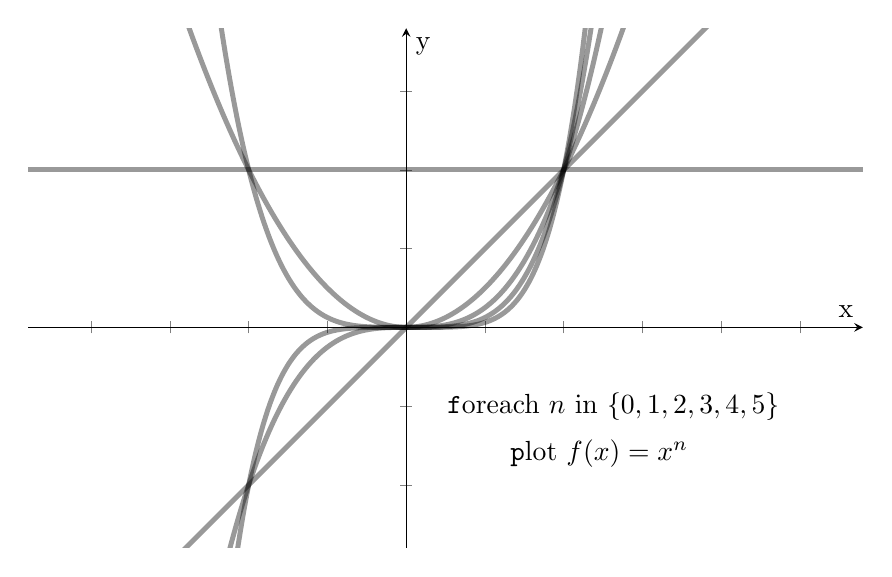
\begin{tikzpicture}
    \begin{axis}[
      scale=2.0,
      x=1.0cm,y=1.0cm,
      axis lines=middle,
      xmin=-2.4,
      xmax=2.9,
      ymin=-1.4,
      ymax=1.9,
      xlabel={x},
      ylabel={y},
      xticklabels={,,},
      yticklabels={,,},
      samples=100]
      \clip(-2.4,-1.4) rectangle (2.9,1.9);
      \addplot[line width=1.8pt,opacity=0.4,smooth,domain=-2.5:3.4] (x,1);
      \foreach \n in {1,2,3,4,5} {
        \addplot[line width=1.8pt,opacity=0.4,smooth,domain=-2.0:2.0] (x,x^\n);
      }
      \draw (0.2,-.5) node[anchor=west] {\texttt foreach $n$ in $\{0,1,2,3,4,5\}$};
      \draw (0.6,-.8) node[anchor=west] {\texttt plot $f(x)=x^n$ };
    \end{axis}
  \end{tikzpicture}
\end{center}
\vspace{-1cm}
\subsection*{Doelstellingen}
{\singlespacing
  Je kan \hfill  {\scriptsize(LP 2005/069, LI 1.2, ET10,11,12,13)}
  \begin{itemize}
  \item vergelijkingen van de eerste, tweede en derde graad in één onbekende oplossen
  \item aan de hand van het functievoorschrift
    \begin{itemize}
    \item een tabel,
    \item het domein,
    \item de nulwaarden,
    \item het tekenverloop,
    \end{itemize}
  \item aan de hand van de grafiek
    \begin{itemize}
    \item domein,
    \item bereik,
    \item nulwaarden
    \item tekenverloop,
    \item stijgen\&dalen,
    \item extrema
    \end{itemize}
    bepalen van veeltermfuncties van de derde graad;
  \item met behulp van ICT de tabel en de grafiek lezen van veeltermfuncties van graad hoger dan drie
  \item veeltermongelijkheden van de eerste, tweede en derde graad in 1 onbekende oplossen, eventueel met behulp van ICT
  \item vraagstukken/problemen oplossen die aanleiding geven tot een veeltermvergelijking, veeltermongelijkheid of veeltermfunctie, eventueel met behulp van ICT
  \end{itemize}
}
\thispagestyle{empty}

\newpage
\tableofcontents
\thispagestyle{empty}
\newpage

\pagenumbering{arabic}
\fancyhead[RO,LE]{Veeltermfuncties}
\fancyhead[RE,LO]{}



\onehalfspacing

\section{Veeltermvergelijkingen}



\subsection{Definitie}

\paragraph{Eenterm}
\begin{mdframed}
Een {\bf eenterm} is een product van een coëfficiënt met een macht van een variabele:
$$ax^n\qquad\qquad\mbox{ met }a\in\mathbb{R}, n\in\mathbb{N}$$
\end{mdframed}

\paragraph{Veelterm}
\begin{mdframed}
  Een {\bf reële veelterm} in de variabele $x$ is een som van ééntermen:
  $$ a_nx^n + a_{n-1}x^{n-1} + \cdots + a_1x + a_0 \;.$$
  De reële getallen $a_n, a_{n-1}, \cdots, a_1, a_0$ noemen we de {\bf coëfficiënten} van de veelterm.
  De hoogste exponent bij de variabele $x$ is de {\bf graad} van de veelterm.
\end{mdframed}

\paragraph{Veeltermvergelijking}
\begin{mdframed}
  Een {\bf veeltermvergelijking} in één onbekende $x$ is een vergelijking die in de vorm
  $$a_nx^n + a_{n-1}x^{n-1} + \cdots + a_1x + a_0 = 0$$
  gebracht kan worden.\\
  De hoogste exponent bij de onbekende $x$ is de {\bf graad} van de veelterm.
\end{mdframed}



\begin{oefening}
  Zijn volgende vergelijkingen veeltermvergelijkingen en zo ja, van welke graad?
  \begin{multicols}{2}
    \begin{enumerate}[(a)]
    \item $2x + 2 = 0$
    \item $\sqrt{3x+1} = 0$
    \item $x^2-3x+8=0$
    \item $x^4=-16$
    \end{enumerate}
  \end{multicols}
\end{oefening}



\paragraph{Oplossen van een veeltermvergelijking}
\begin{mdframed}
  Een veeltermvergelijking {\bf oplossen} is het zoeken naar alle onbekenden $x$ zodat de vergelijking waar wordt.
\end{mdframed}



\begin{oefening}
  Beschouw de vergelijking
  $$x^3-6x^2+5x+12=0\;.$$
  \begin{enumerate}[(a)]
  \item Onderzoek of de gehele getallen van -3 tot 3 aan deze vergelijking voldoen.
  \item Zijn er nog andere getallen die aan deze vergelijking voldoen?
  \end{enumerate}
\end{oefening}



\pagebreak
\subsection{Veeltermvergelijkingen van de eerste graad}

\begin{itemize}
\item Synoniem: eerstegraadsvergelijking, lineaire vergelijking
\item Standaardvorm:
  $$ax + b = 0$$
  met $a, b \in \mathbb{R}$ en $a\neq 0$
\item Oplossing:
  $$V=\{-\dfrac{b}{a}\}$$
\end{itemize}

\paragraph{Werkwijze om een eerstegraadsvergelijking op te lossen}
\begin{enumerate}
\item Haakjes wegwerken
\item Noemers wegwerken
\item Onbekenden links, bekenden rechts
\item Vereenvoudigen
\item Onbekende afzonderen
\item Oplossingenverzameling opschrijven en proef maken
\end{enumerate}




\begin{oefening}
  Los de volgende vergelijkingen van de eerste graad op in $\mathbb{R}$
  \begin{multicols}{2}
    \begin{enumerate}[(a)]
      \itemsep0.7em
    \item $4x-8=0$
    \item $3x+9=0$
    \item $-3x+9=0$
    \item $2(x+6)=4-(x+7)$
    \item $x - \dfrac{x-2}{3} = 4$
    \item $2(x-3)+7=5-(2-x)$
    \item $(x+1)^2-2=x(x-3)-(1-2x)$
    \item $\dfrac{3+2x}{4}-\dfrac{4x-5}{5}=\dfrac{21-6x}{6}$
    \item $\dfrac{4x}{3}-\left(\dfrac{3}{2}-\dfrac{x}{4}\right)=x+4\left(\dfrac{2x}{3}-1\right)$
    \item $\dfrac{3(x-1)}{5}-\dfrac{2(1-4x)}{7}=x+\dfrac{x+1}{5}$
    \item $\dfrac{5x}{8}-\dfrac{x-\frac{5}{2}}{4}=1$
    \item $\dfrac{x}{5}+\dfrac{x}{2}=-7$
    \item $\dfrac{3-x}{4}-\dfrac{x-2}{3}=\dfrac{x}{2}-\dfrac{4x+1}{12}$
    \end{enumerate}
  \end{multicols}
\end{oefening}


\pagebreak
\subsubsection*{Toepassingen}

Volgende oefeningen geven toepassingen waarbij we vergelijkingen van de eerste graad oplossen. Ga steeds als volgt te werk:

\begin{description}
  \item[Onbekende(n)] Wat wordt gevraagd. Hoe kan je dat zo eenvoudig mogelijk uitdrukken.
  \item[Vergelijking(en)] Lees de toepassing heel aandachtig. Probeer de zinnen te vinden waaruit we vergelijking kunnen halen. Vervang geleidelijk aan de zin door een wiskundige uitdrukking. Het is normaal dat je bij deze stap de vraag verschillende keren opnieuw moet lezen.
  \item[Oplossen] Als de vergelijkingen meerdere onbekenden bevatten, probeer dan de vergelijkingen te herschrijven zodat ze maar één onbekende meer bevatten. Los de vergelijking dan op met de geziene methode.
  \item[Antwoord] Kijk naar je oplossingenverzameling en lees de vraag opnieuw. Beantwoord nu specifiek op het gevraagde.
\end{description}



\begin{oefening}
Twee getallen hebben als som 60. De som van de helft van het eerste getal en een derde van het tweede getal is 20. Bepaal die getallen.
\end{oefening}

\begin{oefening}
We gaan naar de bakker en geven in totaal 12.60 euro uit voor chocoladekoeken en croissants. We weten dat een chocoladekoek 0.65 euro en een croissant 0.60 euro kost. Hoeveel chocoladekoeken hebben we mee?
\end{oefening}

\begin{oefening}
De energieprijs voor elektriciteit is 0.25 euro per kWh tijdens de dag en 0.15 euro per kWh tijdens de nacht. De maandelijkse distributiekost is 22.50 euro.
\begin{enumerate}[(a)]
  \item Wat betaal je als je enkel tijdens de dag stroom verbruikt en in het totaal voor één maand 350 kWh stroom hebt gebruikt?
  \item Stel, je factuur is 124.30 euro en je hebt deze maand 548 kWh aan stroom verbruikt. Hoeveel verbruikte je tijdens de dag en tijdens de nacht?
\end{enumerate}
\end{oefening}

\begin{oefening}
Aron gaat om de twee dagen trainen met zijn koersfiets. Hij begint de maandag en traint een ganse week. In het totaal fietst hij $280 \km$. Elke volgende trainingsdag fietst hij $20 \km$ meer dan de vorige. Hoeveel kilometer zal hij de zondag fietsen?
\end{oefening}

\vfill
\hfill
\begin{tikzpicture}[remember picture, overlay]
    \hspace*{-2cm}
        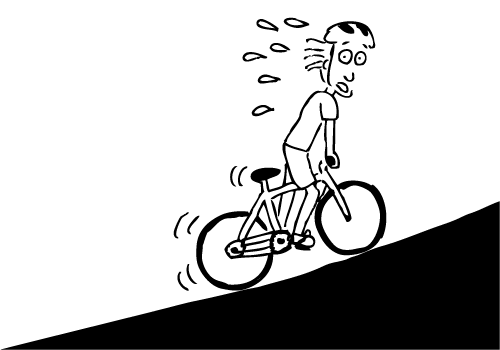
\includegraphics[width=4cm]{fietser}
\end{tikzpicture}



\pagebreak
\subsection{Veeltermvergelijkingen van de tweede graad}

\begin{itemize}
\item Synoniem: tweedegraadsvergelijking, vierkantsvergelijking, kwadratische vergelijking
\item Standaardvorm:
  $$ax^2 + bx + c = 0$$
  met $a, b, c \in \mathbb{R}$ en $a\neq 0$
\item Volledige tweedegraadsvergelijking:\\
  We noemen een tweedegraadsvergelijking {\bf volledig} als alle coëfficiënten verschillend van nul zijn, d.w.z. als
  $$ a\neq 0 \qquad b\neq 0 \qquad c\neq 0$$
\item Oplossen m.b.v. de discriminantmethode:
  \begin{itemize}
  \item Bereken de discriminant $D=b^2-4ac$
  \item Drie gevallen:
    \begin{itemize}
    \item als $D<0$, dan zijn er geen oplossingen
      $$V=\emptyset$$
    \item als $D>0$, dan zijn er twee verschillende oplossingen: $x_{1,2}=\dfrac{-b\pm\sqrt{D}}{2a}$
      $$V=\{x_1, x_2\}$$
    \item als $D=0$, dan heeft de vergelijking één oplossing (eigenlijk twee samenvallende oplossingen)
      $$V=\{\dfrac{-b}{2a}\}$$
    \end{itemize}
  \end{itemize}
\item Onvolledige tweedegraadsvergelijking:\\
  Een tweedegraadsvergelijking is {\bf onvolledig} als $b=0$ of $c=0$ is. Onvolledige tweedegraadsvergelijkingen kunnen als volgt eenvoudig opgelost worden:
  \begin{itemize}
    \item $b=0$ en $c=0$, dus $ax^2=0$, dan kan $x$ enkel de waarde nul hebben, dus $V=\{0\}$
    \item $b=0$, dus $ax^2+c=0\LRA x^2=\dfrac{-c}{a}$, dus er zijn twee oplossingen als $\dfrac{-c}{a}$ positief is, dus $V=\{-\sqrt{\dfrac{-c}{a}}, +\sqrt{\dfrac{-c}{a}}\}$
    \item $c=0$, dus $ax^2+bx=0\LRA x(ax+b)=0$, dus er zijn altijd twee oplossingen namelijk $x=0$ en de oplossing van de eerstegraadsvergelijking $ax+b=0$, dus $V=\{0, -\dfrac{b}{a}\}$
  \end{itemize}
\end{itemize}



\begin{oefening}
  Los de volgende vergelijkingen van de tweede graad op in $\mathbb{R}$
  \begin{multicols}{2}
    \begin{enumerate}[(a)]
      \itemsep0.7em
    \item $2x^2-4x-6=0$
    \item $5x(x-2)=x(3x-4)-5$
    \item $\frac{2}{3}x^2+5x+1=0$
    \item $80x^2+8x=15$
    \item $80x^2+15=-8x$
    \item $(3-x)(3+x)=(x-4)^2$
    \item $(x-2)^2=x^2-4$
    \item $(3x+2)(3x-2)+6x+5=0$
    \item $x+1=(x+1)(x-1)$
    \item $4x^2-20x+25=0$
    \item $3x^2+5=0$
    \item $x=x^2$
    \item $2\left(7x+32\right)=(3x+8)^2$
    \item $11x+13=2x^2$
    \item $x\left(x+3\right)+2\left(5+2x\right)=0$
    \item $x^2+2x-8=0$
    \item $(x+3)^2=16$
    \item $9x^2+30x+25=0$
    \item $10x^2+7x-3=0$
    \item $x^2=x+1$
    \item $37x^2+13x-50=0$
    \item $3x(3x+10)+5=-20$
    \item $x^2=3x-18$
    \item $x^2=10x-25$
    \end{enumerate}
  \end{multicols}
\end{oefening}

\begin{oefening}
  Los op in $\mathbb{R}$
  \begin{enumerate}[(a)]
      \itemsep1em
    \item $x^2+x-8=(x-6)^2$ \tabto{6cm} {\color{gray}$V=\{\dfrac{44}{13}\}$}
    \item $x^2+\dfrac{15}{2}=\dfrac{11x}{2}$ \tabto{6cm} {\color{gray}$V=\{\dfrac{5}{2}, 3\}$}
    \item $(2x-4)(2x+4)=(x+2)^2$ \tabto{6cm} {\color{gray}$V=\{-2,\dfrac{10}{3}\}$}
    \item $9x^2-36=(6+3x)^2$ \tabto{6cm} {\color{gray}$V=\{-2\}$}
    \item $19-x+x^2=18-2x-x^2$ \tabto{6cm} {\color{gray}$V=\{\}$}
    \item $25x^2+20x=-9$ \tabto{6cm} {\color{gray}$V=\{-\dfrac{3}{5}\}$}
    \item $6x^2=x+1$ \tabto{6cm} {\color{gray}$V=\{-\dfrac{1}{3},\dfrac{1}{2}\}$}
  \end{enumerate}
\end{oefening}



\pagebreak
\subsection*{Toepassingen}



\begin{oefening}
We gooien een bal recht omhoog. De begin hoogte is dan $1.75 \m$. We doen dit met een snelheid van $17 \mpers$. Na hoeveel seconden zal de bal op de grond terecht komen?

Als we de luchtweerstand negeren kunnen we de hoogte op elk tijdstip bepalen door volgende informatie op te tellen:
\begin{itemize}
  \item De starthoogte
  \item De startsnelheid vermenigvuldigd met de tijd
  \item De kracht van de gravitatie, deze is steeds $-5t^2\approx -\frac{at^2}{2}$ met $a=9.811\mpers^2$.
\end{itemize}
\end{oefening}

\begin{oefening}
De ring links en de cirkel rechts hebben dezelfde oppervlakte. Bepaal $x$.
\begin{center}
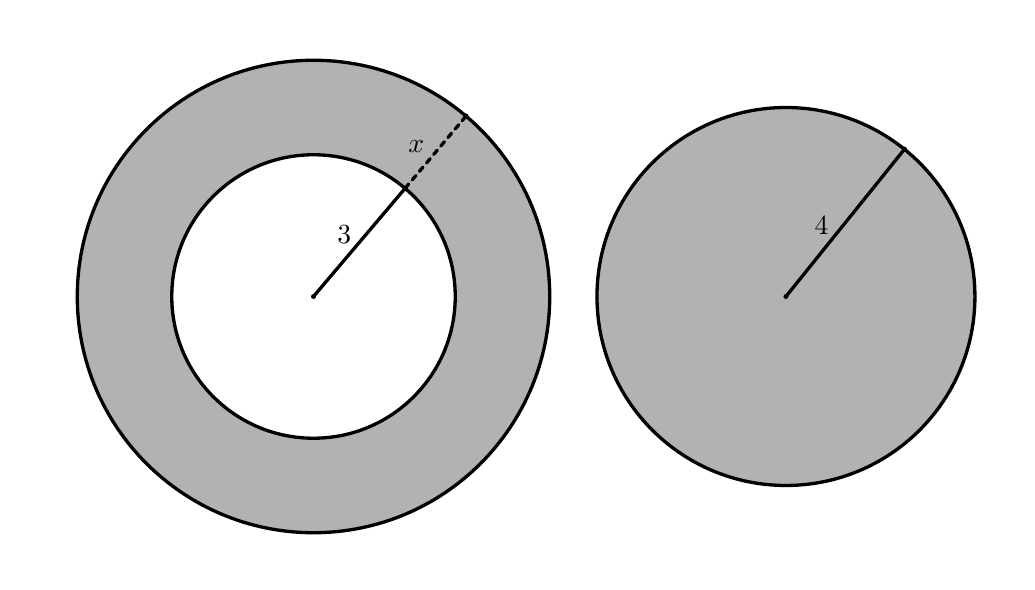
\begin{tikzpicture}[scale=0.6, line cap=round,line join=round,>=triangle 45,x=1.0cm,y=1.0cm]
\clip(-2.05,-0.62) rectangle (18.68,10.69);
\draw [line width=1.2pt,fill=gray!60] (4,5) circle (5cm);
\draw [line width=1.2pt,fill=white] (4,5) circle (3cm);
\draw [line width=1.2pt,fill=gray!60] (14,5) circle (4cm);
\draw [line width=1.2pt] (14,5)-- (16.51,8.12);
\draw [line width=1.2pt] (4,5)-- (5.94,7.29);
\draw [line width=1.2pt,dash pattern=on 2pt off 2pt] (5.94,7.29)-- (7.23,8.82);
\draw (5.8,8.5) node[anchor=north west] {$x$};
\draw (4.3,6.7) node[anchor=north west] {3};
\draw (14.4,6.9) node[anchor=north west] {4};
\fill [color=black] (4,5) circle (1.5pt);
\fill [color=black] (14,5) circle (1.5pt);
\fill [color=black] (7.23,8.82) circle (1.5pt);
\fill [color=black] (16.51,8.12) circle (1.5pt);
\fill [color=black] (5.94,7.29) circle (1.5pt);
\end{tikzpicture}
\end{center}
\end{oefening}



\pagebreak
\subsection{Veeltermvergelijkingen van graad $\geq 3$}

Veeltermvergelijkingen van hogere graad kunnen we oplossen door handmatig (m.b.v. een ZRM) één oplossing $x=a$ te zoeken waardoor we van de veelterm een deler $x-a$ kunnen afsplitsen. De restveelterm kan gevonden worden m.b.v. het {\bf algoritme van Horner}.

\paragraph{Voorbeeld}

We lossen de vergelijking $$x^3-4x^2+x+6=0$$ op.

\begin{itemize}
\item Zoek een $x$ zodat de vergelijking waar wordt:
  \begin{description}
  \item[$x=1$] $\rightarrow 1^3-4\cdot 1^2+1+6 = 4 \neq 0$
  \item[$x=0$] $\rightarrow 0^3-4\cdot 0^2+0+6 = 6 \neq 0$
  \item[$x=-1$] $\rightarrow (-1)^3-4\cdot (-1)^2+(-1)+6 = 0$
  \end{description}
\item Dus $x=-1$ is een oplossing. Dit wil zeggen dat $x-(-1)$ of korter $x+1$ een deler is van de de veelterm. We herschrijven de vergelijking:
  \begin{eqnarray*}
    x^3-4x^2+x+6&=&0\\
    \LRA (x+1)\underbrace{(\qquad ? \qquad)}_{\mbox{restveelterm}}&=&0\\
  \end{eqnarray*}
\item De restveelterm vinden we m.b.v. het algoritme van Horner:
  \begin{center}
    \begin{tabular}{c|cccc}
      & 1 & -4 & 1 & 6\\
      -1 & $\downarrow$ & -1 & 5 & -6\\
      \hline
      & 1 & -5 & 6 & 0
    \end{tabular}
  \end{center}
\item We krijgen dus:
  \begin{eqnarray*}
    x^3-4x^2+x+6&=&0\\
    \LRA (x+1)(x^2-5x+6)&=&0\\
  \end{eqnarray*}
\item Voor de factor $(x+1)$ hebben we reeds de oplossing $x_0=-1$ gevonden. Ook de factor $(x^2-5x+6)$ heeft oplossingen. Deze vinden we m.b.v. de discriminantmethode:
  $$x^2-5x+6=0$$
  $$D=25-4\cdot 1\cdot 6=1$$
  $$x_{1,2}=\dfrac{5\pm 1}{2}=3\mbox{ en }2$$
\item Dus $x^3-4x^2+x+6=0$ heeft als oplossingenverzameling
  $$V=\{-1, 2, 3\}$$
\end{itemize}



\begin{oefening}
  Los op in $\mathbb{R}$
  \begin{multicols}{2}
    \begin{enumerate}[(a)]
    \itemsep0.7em
    \item $x^3+2x-3=0$
    \item $7x^3+8x^2+3x+2=0$
    \item $x^3-x+6=0$
    \item $3x^2(x-1)=\dfrac{7}{2}x^2-2$
    \item $8x^3+12x^2+6x+2=0$
    \item $20x^3+60x^2+45x=0$
    \item $x^4-4x^3-x^2+16x-12=0$
    \item $x+\dfrac{7x}{2}=\dfrac{3x^3}{2}+\dfrac{3x^2}{2}+\dfrac{3}{2}$
    \item $x^3+(2x+1)^2=x+1$
    \end{enumerate}
  \end{multicols}
\end{oefening}

\begin{oefening} % www3.ul.ie/~mlc/support/.../chap3/3_3.pdf
  Los volgende vergelijkingen van graad hoger dan twee op in $\mathbb{R}$:
  \begin{multicols}{2}
  \begin{enumerate}[(a)]
  \itemsep.7em
  \item $x^3-17x^2+54x-8=0$
  \item $x^3-6x^2+11x-6=0$
  \item $x^3-7x=6$
  \item $2x^3+9x^2+7x+2=2x^2$
  \item $22x+8=3x^3+7x^2$
  \item $2x^4+8x^3-\dfrac{7x^2}{2}-\dfrac{67x}{2}-15=0$
  \item $4x^4+8x^3+3x^2-2x-1=0$
  \end{enumerate}
  \end{multicols}
\end{oefening}

\begin{oefening}
Los op in $\mathbb{R}$:
\begin{enumerate}[(a)]
  \itemsep0.6em
  \begin{multicols}{2}
  \item $2x^3+3x^2-17x+12=0$
  \item $3x^3+13x^2-18x-40=0$
  \item $x^3+4x^2-15x-18=0$
  \item $2x^3+9x^2+7x-6=0$
  \item $-3x^3+16x^2-17x+4=0$
  \item $2x^4+3x^3=17x^2-12x$
  \item $16x^3+4x=3x^4+17x^2$
  \item $2x^4-11x^3-12x^2+36x=0$
  \item $x^4+3x^3-51x^2+37x+90=0$
  \item $6x^3-11x^2-3x+2=0$
  \item $x^3-9x^2+26x=24$
  \item $x^3-3x+2=0$
  \item $x^4+x^3=10x^2-8x$
  \item $x^4+2x-1=2x^3$
  \item $1=x^4$
  \item $3x^2+x(x-1)^2=5x+4$
  \item $(x+1)(x^2+2x+1)=2x(x+2)-1$
  \item $x^3+70=39x$
  \item $x^4+3x^2+10x=6x^3$
  \item $-2(10x+x^3)=x^2(10+x^2)$
  \item $x^4+82x+176=93x^2-2x^3$
  \item $12x^3+22x^2-6x-4=0$
  \item $2x(3x^3-26)=20+x^2(31-7x)$
  \item $x^4-8x^3-3x^2+62x+56=0$
  \item $-x^3+3x^2-3x=0$
  \item $-x^4-x^3-7x^2-9x+18=0$
  \end{multicols}
\end{enumerate}
\end{oefening}


\pagebreak
\subsection{Veeltermvergelijkingen oplossen m.b.v. Geogebra}

\subsection*{Eerste methode}

\paragraph*{Voorbeeld:} Los op in $\mathbb{R}$
$$x^3-2x^2-1=x^2+x-4$$

Beschouw het linkerlid en het rechterlid als functies:
$$f(x)=x^3-2x^3-1$$
$$g(x)=x^2+x-4$$

Voor alle $x$ die een oplossing zijn van de originele vergelijk geldt dus dat
$$f(x)=g(x)$$

Construeer nu de grafieken van $f(x)$ en van $g(x)$ met Geogebra. Download het programma op \url{https://www.geogebra.org/} als dit nog niet geïnstalleerd is. Hiervoor moet je onderaan in het commandovenster het commando \verb#f(x)=x^3-2*x^3-1# en \verb#g(x)=x^2+x-4# invoeren.

Voor de snijpunten van de grafieken geldt nu dus dat $f(x)=g(x)$. En we zoeken de $x$-waarden om de originele vergelijking waar te maken. In het menu van Geogebra moeten we dus op zoek naar het icoon om het snijpunt van de twee grafieken te bepalen. Eenmaal dat we alle snijpunten hebben moeten we maar enkel de verschillende $x$-waarden van deze punten aflezen om de oplossingenverzameling te bepalen:

$$V=\{-1, 1, 3\}$$

\subsection*{Tweede methode}

\paragraph*{Voorbeeld:} Los op in $\mathbb{R}$
$$x^3-2x^2-1=x^2+x-4$$

We herschrijven deze vergelijking eerst in zijn standaardvorm:
$$\LRA x^3-3x^2-x + 3=0$$

We hoeven nu enkel het linkerlid als de functie
$$f(x)=x^3-3x^2-x + 3$$
te plotten. Want als we naar de vergelijking in standaardvorm kijken zoeken we eigenlijk de nulwaarden van deze functie.

Construeer de grafiek van deze functie $f$ in Geogebra en lees de nulwaarde af via het menu snijpunten van 2 objecten. Je zou dezelfde oplossingenverzameling

$$V=\{-1, 1, 3\}$$

moeten vinden.



\begin{oefening}
  Los op in $\mathbb{R}$\\
  \begin{enumerate}[(a)]
    \itemsep2em
  \item $\displaystyle\frac{{x}^{6}}{2}+\frac{21\,{x}^{5}}{4}+\frac{81\,{x}^{4}}{4}+\frac{67\,{x}^{3}}{2}+18\,{x}^{2}=\frac{27\,x}{4}+\frac{27}{4}$
  \item $\displaystyle{x}^{3}+\frac{7\,{x}^{2}}{2}+x=\frac{3}{2}$
  \end{enumerate}
\end{oefening}

\begin{oefening}
  Los volgende vergelijkingen op in $\mathbb{R}$ door gebruik te maken van Horner, controleer daarna je antwoord m.b.v. ICT.\\
  \begin{enumerate}[(a)]
    \itemsep1em
  \item $\displaystyle{x}^{3}+{x}^{2}=2\,x$
  \item $\displaystyle{x}^{6}-{x}^{5}-13\,{x}^{4}=-13\,{x}^{3}-36\,{x}^{2}+36\,x$
  \end{enumerate}
\end{oefening}

\begin{oefening}
  Maak gebruik van Geogebra om de volgende vergelijkingen op te lossen in $\mathbb{R}$
  \begin{multicols}{2}
    \begin{enumerate}[(a)]
      \itemsep0.7em
    \item $-5x+4=0$
    \item $2(x+6)=4-(x+7)$
    \item $2x^2-4x-6=0$
    \item $5x(x-2)=x(3x-4)-5$
    \item $3x^3+x^2-8x+4=0$
    \item $x^3+6x^2-x-30=0$
    \item $x^3-3x^2+4=0$
    \item $-4(x-5)=3(2x+1)$
    \item $(x+\sqrt{5})(x^2+2x-8)=0$
    \item $5x^2+3x-4=0$
    \end{enumerate}
  \end{multicols}
\end{oefening}


\pagebreak
\section{Veeltermfuncties}



\subsection{Definities}

\paragraph*{Veeltermfunctie}
\begin{mdframed}
  Een {\bf veeltermfunctie} is een reële functie waarvan het functievoorschrift gegeven wordt door een veelterm:
  $$f(x)= a_nx^n + a_{n-1}x^{n-1} + \cdots + a_1x + a_0$$
\end{mdframed}

De {\bf graad van de veeltermfunctie} is gelijk aan de graad van de veelterm. In de definitie is de veeltermfunctie dus van de $n$-de graad.



\begin{oefening}
  Welke van de volgende functies zijn veeltermfuncties. Als het veeltermfuncties zijn, wat is dan hun graad?
\begin{multicols}{2}
  \begin{enumerate}[(a)]
  \itemsep1em
  \item $f(x)=\dfrac{2}{3}x+2$
  \item $f(x)=0.5x^2-x-1.5$
  \item $f(x)=\sqrt{3x^2+2x-6}$
  \item $f(x)=-\dfrac{3}{4}x^2+3x$
  \item $f(x)=\dfrac{3}{x^2}+\dfrac{2}{x}+1$
  \item $f(x)=42$
  \item $f(x)=3x^2-0.5x^3$
  \item $f(x)=2^x+2$
  \end{enumerate}
\end{multicols}
\end{oefening}

\begin{oefening}
Schrijf volgende veeltermfuncties in hun standaardvorm.
\begin{multicols}{2}
  \begin{enumerate}[(a)]
  \itemsep1em
  \item $f(x)=2+x^3-x^2$
  \item $f(x)=-(x^2-2x+3)$
  \item $f(x)=3x(x^2-2x+3)$
  \item $f(x)=(x-2)(x+3)$
  \item $f(x)=(x-2)^2$
  \item $f(x)=(2x-3)^2$
  \item $f(x)=(x^2+2x)^2$
  \item $f(x)=(2x-4)^3$
  \item $f(x)=\dfrac{1}{7}(x-2)^2$
  \item $f(x)=\dfrac{x+2}{3}\cdot\dfrac{x-2}{2}$
  \end{enumerate}
\end{multicols}
\end{oefening}


\pagebreak
\subsection{Veeltermfuncties van graad 0}

\begin{itemize}
\item Synoniemen voor deze functies zijn nulveeltermfuncties of {\bf constante functies}. Wij zullen vanaf nu de benaming constante functie gebruiken.
\item Deze functies hebben de vorm
  $$f(x) = a$$
  met $a$ een reëel getal.
\item De grafiek van deze functie is een horizontale rechte evenwijdig met de $x$-as.
\item Het domein is dus $\mathbb{R}$
\item De grafiek van deze functie snijdt de $y$-as in het punt $(0, a)$.
\item Als $a\neq 0$ dan heeft deze functie geen nulwaarden.
\item Als $a=0$ dan heeft deze functie alle reële getallen als nulwaarden.
\end{itemize}



\begin{oefening}
  Beschouw de functie
  $$f(x)=-2\;.$$
  \begin{enumerate}[(a)]
  \item Dit is een veeltermfunctie van de hoeveelste graad?
  \item Hoe noemen we zulk een functie?
  \item Hoe ziet deze functie eruit?
  \item Wat zijn de nulwaarden?
  \item Teken de grafiek zonder een functiewaardentabel te maken.
  \end{enumerate}
\end{oefening}



\paragraph*{Constante functie bespreken}
\begin{mdframed}
  \begin{itemize}
  \item Functievoorschrift: $f(x)=a$
  \item $\dom f = \mathbb{R}$ en $\ber f = \{a\}$
  \item Nulwaarden:
    \begin{itemize}
    \item Als $a\neq 0$ dan geen nulwaarden.
    \item Als $a=0$ dan zijn de nulwaarden $\mathbb{R}$.
    \end{itemize}
  \item Tekenverloop:
    \begin{center}
      \begin{tabular}{c|lcr}
        $x$ & $-\infty$ & & $+\infty$\\
        \hline
        $f(x)$ & & teken van $a$ &
      \end{tabular}
    \end{center}
  \item Functiewaardentabel en grafiek: /
  \end{itemize}
\end{mdframed}

\begin{oefening}
  Beschrijf volgende constante functies:
  \begin{enumerate}[(a)]
  \item $f(x)=42$
  \item $f(x)=0$
  \end{enumerate}
\end{oefening}

\begin{oefening}
  Geef het functievoorschrift van de rechte die door de punten $(-2,1.5)$ en $(3,1.5)$ gaat.
\end{oefening}

\begin{oefening}
  Geef het functievoorschrift van de volgende grafiek:
  \begin{center}
    \definecolor{cqcqcq}{rgb}{0.75,0.75,0.75}
    \begin{tikzpicture}[scale=0.7,line cap=round,line join=round,>=triangle 45,x=1.0cm,y=1.0cm]
      \draw [color=cqcqcq,dash pattern=on 1pt off 1pt, xstep=2.0cm,ystep=2.0cm] (-4.62,-4.36) grid (8.32,4.42);
      \draw[->,color=black] (-4.62,0) -- (8.32,0);
      \foreach \x in {-4,-2,2,4,6,8}
      \draw[shift={(\x,0)},color=black] (0pt,2pt) -- (0pt,-2pt) node[below] {\footnotesize $\x$};
      \draw[->,color=black] (0,-4.36) -- (0,4.42);
      \foreach \y in {-4,-2,2,4}
      \draw[shift={(0,\y)},color=black] (2pt,0pt) -- (-2pt,0pt) node[left] {\footnotesize $\y$};
      \draw[color=black] (0pt,-10pt) node[right] {\footnotesize $0$};
      \clip(-4.62,-4.36) rectangle (8.32,4.42);
      \draw[line width=2pt, smooth,samples=100,domain=-4.620000000000001:8.320000000000006] plot(\x,{0-3});
      \draw (4.74,-3.0) node[anchor=south] {$f(x)$};
    \end{tikzpicture}
  \end{center}
\end{oefening}

\pagebreak
\subsection{Veeltermfuncties van graad 1}

\begin{itemize}
\item Synoniemen voor deze functies zijn {\bf eerstegraadsfuncties} of lineaire functies. Wij zullen vanaf nu de benaming eerstegraadsfunctie gebruiken.
\item Deze functies hebben de vorm
  $$f(x) = ax+b $$
  met $a$ en $b$ een reëel getallen en $a$ verschillend van $0$.
\item De grafiek van deze functie is een schuine rechte die stijgt indien $a > 0$ en daalt indien $a<0$.
\item De coëfficiënt $a$ wordt de richtingscoëfficiënt genoemd, het is een maat voor de helling van de rechte ten opzichte van de $x$-as.
\item Het domein is dus $\mathbb{R}$.
\item De grafiek van deze functie snijdt de $x$-as in het punt $(-\dfrac{b}{a}, 0)$ en $x_0=-\dfrac{b}{a}$ is de enige nulwaarde van de functie.
\item De grafiek van deze functie snijdt de $y$-as in het punt $(0, b)$. De constante term $b$ bepaalt dus waar de grafiek de $y$-as snijdt.
\item De grafiek van deze functie heeft geen extrema.
\end{itemize}



\begin{oefening}
  Beschouw de functie
  $$f(x)=-\dfrac{1}{2}x+2\;.$$
  \begin{enumerate}[(a)]
  \item Dit is een veeltermfunctie van de hoeveelste graad?
  \item Hoe noemen we zulk een functie?
  \item Hoe ziet deze functie eruit?
  \item Wat zijn de nulwaarden?
  \item Waar snijdt deze functie de assen?
  \item Teken de grafiek zonder een functiewaardentabel te maken.
  \end{enumerate}
\end{oefening}



\paragraph*{Eerstegraadsfunctie bespreken}
\begin{mdframed}
  \begin{itemize}
  \item Functievoorschrift: $f(x)=ax + b$
  \item $\dom f = \mathbb{R}$ en $\ber f = \mathbb{R}$
  \item Nulwaarde: $x_0=-\dfrac{b}{a}$
  \item Tekenverloop:
    \begin{center}
      \begin{tabular}{c|lp{2.5cm}cp{1.5cm}r}
        $x$ & $-\infty$ & & $x_0$ & & $+\infty$\\
        \hline
        $f(x)$ & & tegengesteld teken van $a$ & 0 & teken van $a$ &
      \end{tabular}
    \end{center}
  \item Functiewaardentabel: twee, hoogstens drie koppels is voldoende
  \item Grafiek maken
  \item Stijgen\&dalen:\\
    \begin{minipage}{0.45\textwidth}
      \centering $a>0$\\
      \begin{tabular}{c|lcr}
        $x$ & $-\infty$ & & $+\infty$\\
        \hline
        $f(x)$ & & $\nearrow$ &
      \end{tabular}
    \end{minipage}
    \begin{minipage}{0.45\textwidth}
      \centering $a<0$\\
      \begin{tabular}{c|lcr}
        $x$ & $-\infty$ & & $+\infty$\\
        \hline
        $f(x)$ & & $\searrow$ &
      \end{tabular}
    \end{minipage}
  \end{itemize}
\end{mdframed}



\begin{oefening}
  Bespreek volgende eerstegraadsfuncties:
  \begin{enumerate}[(a)]
  \item $f(x)=2x-3$
  \item $f(x)=-x+4$
  \end{enumerate}
\end{oefening}

\begin{oefening}
  Bepaal het functievoorschrift van
  \begin{enumerate}[(a)]
  \item de rechte door $(-2, 3)$ en $(1, 0)$.
  \item de rechte door $(-2, 0)$ en $(1, 3)$.
  \item de rechte door $(1, -1)$ en $(3, -1)$.
  \item de rechte door $(3, -1)$ en $(3, 6)$.
  \end{enumerate}
\end{oefening}

\begin{oefening}
  Teken de grafiek van de eerstegraadsfunctie die als nulwaarde $x=3$ heeft en die de $y$-as snijdt in het punt $(0,-6)$. Kan je het functievoorschrift vinden voor deze functie?
\end{oefening}

\begin{oefening}
  Geef het functievoorschrift van de volgende grafiek:
  \begin{center}
    \definecolor{cqcqcq}{rgb}{0.75,0.75,0.75}
    \begin{tikzpicture}[scale=0.75, line cap=round,line join=round,>=triangle 45,x=1.0cm,y=1.0cm]
      \draw [color=cqcqcq,dash pattern=on 1pt off 1pt, xstep=2.0cm,ystep=2.0cm] (-4.54,-2.74) grid (8.56,4.62);
      \draw[->,color=black] (-4.54,0) -- (8.56,0);
      \foreach \x in {-4,-2,2,4,6,8}
      \draw[shift={(\x,0)},color=black] (0pt,2pt) -- (0pt,-2pt) node[below] {\footnotesize $\x$};
      \draw[->,color=black] (0,-2.74) -- (0,4.62);
      \foreach \y in {-2,2,4}
      \draw[shift={(0,\y)},color=black] (2pt,0pt) -- (-2pt,0pt) node[left] {\footnotesize $\y$};
      \draw[color=black] (0pt,-10pt) node[right] {\footnotesize $0$};
      \clip(-4.54,-2.74) rectangle (8.56,4.62);
      \draw[line width=2pt, smooth,samples=100,domain=-4.540000000000001:8.560000000000006] plot(\x,{0-0.5*(\x)+3});
      \draw (0.68,3.22) node[anchor=north west] {$f$};
    \end{tikzpicture}
  \end{center}
\end{oefening}

\pagebreak
\subsection{Veeltermfuncties van graad 2}

\begin{itemize}
\item Synoniemen voor deze functies zijn {\bf tweedegraadsfuncties} of kwadratische functies. Wij zullen vanaf nu de benaming tweedegraadsfunctie gebruiken.
\item Deze functies hebben de vorm
  $$f(x) = ax^2+bx+c $$
  met $a$, $b$ en $c$ een reëel getallen en $a$ verschillend van $0$.
\item We kunnen voor elke reële waarde de functiewaarde bereken, dus het domein is $\mathbb{R}$.
\item De grafiek van deze functie is een parabool met symmetrieas evenwijdig met de $y$-as.
\item Als $a>0$ dan opent de parabool zich naar boven en dat noemen we een {\bf dalparabool}.
\item Als $a<0$ dan opent de parabool zich naar beneden en dat noemen we een {\bf bergparabool}.
\item De top van de parabool bevindt zich in het punt $(-\dfrac{b}{2a}, f(-\dfrac{b}{2a}))$. Dit punt kan ook berekend worden met $(-\dfrac{b}{2a}, -\dfrac{D}{4a})$, waarbij we $D=b^2-4ac$ de discriminant noemen.
\item De top is het extrema van de functie, een maximum als $a<0$ en een minimum als $a>0$.
\item Een tweedegraadsfunctie kan $0, 1$ of $2$ nulwaarden hebben, afhankelijk van de discriminant.
\end{itemize}



\begin{oefening}
  Beschouw de functie
  $$f(x)=x^2-x-6\;.$$
  \begin{enumerate}[(a)]
  \item Dit is een veeltermfunctie van de hoeveelste graad?
  \item Hoe noemen we zulk een functie?
  \item Hoe ziet deze functie eruit?
  \item Wat zijn de nulwaarden?
  \item Waar snijdt deze functie de assen?
  \item Heeft deze functie een extremum, waar ligt dit extremum en hoe noemen we dit extremum in deze context?
  \item Teken de grafiek zonder een functiewaardentabel te maken.
  \end{enumerate}
\end{oefening}



\pagebreak
\paragraph*{Tweedegraadsfuncties bespreken}
\begin{mdframed}
  \begin{itemize}
  \item Functievoorschrift: $f(x)=ax^2 + bx + c$
  \item $a>0$ dan een dalparabool, $a<0$ dan een bergparabool
  \item $\dom f = \mathbb{R}$
  \item $a>0$ dan $\ber f = [f(-\dfrac{b}{2a}), +\infty]$, $a<0$ dan $\ber f = [-\infty, f(-\dfrac{b}{2a})]$
  \item Nulwaarden: $ax^2+bx+c=0$
    \renewcommand{\labelitemii}{$\bullet$}
    \begin{itemize}
    \item $D=b^2-4ac$
    \item $D>0$ dan twee verschillende nulwaarden $x_1=\dfrac{-b-\sqrt{D}}{2a}$ en $x_0=\dfrac{-b+\sqrt{D}}{2a}$
    \item $D=0$ dan één nulwaarde $x_0=-\dfrac{b}{2a}$
    \item $D<0$ dan geen nulwaarden
    \end{itemize}
  \item Tekenverloop:
    \begin{itemize}
    \item $D>0$
      \begin{tabular}{c|p{1.5cm}cp{2.5cm}cp{1.5cm}}
        $x$ & & $x_1$ & & $x_2$ &\\
        \hline
        $f(x)$ & teken van $a$ & 0 & tegengesteld teken van $a$ & 0 & teken van $a$
      \end{tabular}
    \item $D=0$
      \begin{tabular}{c|lp{1.5cm}cp{1.5cm}r}
        $x$ & $-\infty$ & & $x_0$ & & $+\infty$\\
        \hline
        $f(x)$ & & teken van $a$ & 0 & teken van $a$ &
      \end{tabular}
    \item $D<0$
      \begin{tabular}{c|lcr}
        $x$ & $-\infty$ &  & $+\infty$\\
        \hline
        $f(x)$ & & teken van $a$ &
      \end{tabular}
    \end{itemize}
  \item Functiewaardentabel: kies de nulwaarden en nog een aantal $x$-waarden daarrond
  \item Grafiek maken
  \item Stijgen\&dalen:\\
    \begin{minipage}{0.45\textwidth}
      \centering $a>0$\\
      \begin{tabular}{c|lcr}
        $x$ &  & $-\dfrac{b}{2a}$ & \\[0.1cm]
        \hline
        $f(x)$ & $\searrow$ & $\underset{=f(-\frac{b}{2a})}{\mbox{min}}$ & $\nearrow$
      \end{tabular}
    \end{minipage}
    \begin{minipage}{0.45\textwidth}
      \centering $a<0$\\
      \begin{tabular}{c|lcr}
        $x$ &  & $-\dfrac{b}{2a}$ & \\[0.1cm]
        \hline
        $f(x)$ & $\nearrow$ & $\underset{=f(-\frac{b}{2a})}{\mbox{max}}$ & $\searrow$
      \end{tabular}
    \end{minipage}
  \end{itemize}
\end{mdframed}



\begin{oefening}
  Bespreek de volgende functies:
  \begin{multicols}{2}
  \begin{enumerate}[(a)]
  \item $f(x)=x^2+x-6$
  \item $f(x)=x^2+2x+1$
  \item $f(x)=x^2+4$
  \item $f(x)=3x-2$
  \item $f(x)=-2x^2-3x+1$
  \item $f(x)=4x^2-4x-15$
  \item $f(x)=(x+2)^2-4$
  \item $f(x)=4x+(x-2)^2$
  \item $f(x)=(x-2)(x+2)$
  \item $f(x)=(x+3)^2+(x-3)^2$
  \item $f(x)=-(x-1)(x+1)$
  \item $f(x)=-2x^2+29x-102$
  \end{enumerate}
  \end{multicols}
\end{oefening}

\begin{oefening}
  Zoek het functievoorschrift van de functie $f$ die door de punten $(-1,0)$, $(0,3)$, $(1,4)$ en $(3,0)$ gaat, zie onderstaande grafiek.
  \begin{center}
    \definecolor{cqcqcq}{rgb}{0.75,0.75,0.75}
    \begin{tikzpicture}[scale=0.9, line cap=round,line join=round,>=triangle 45,x=1.0cm,y=1.0cm]
      \draw [color=cqcqcq,dash pattern=on 1pt off 1pt, xstep=1.0cm,ystep=1.0cm] (-2.55,-2.69) grid (5.45,5.36);
      \draw[->,color=black] (-2.55,0) -- (5.45,0);
      \foreach \x in {-2,-1,1,2,3,4,5}
      \draw[shift={(\x,0)},color=black] (0pt,2pt) -- (0pt,-2pt) node[below] {\footnotesize $\x$};
      \draw[->,color=black] (0,-2.69) -- (0,5.36);
      \foreach \y in {-2,-1,1,2,3,4,5}
      \draw[shift={(0,\y)},color=black] (2pt,0pt) -- (-2pt,0pt) node[left] {\footnotesize $\y$};
      \draw[color=black] (0pt,-10pt) node[right] {\footnotesize $0$};
      \clip(-2.55,-2.69) rectangle (5.45,5.36);
      \draw[line width=2pt, smooth,samples=100,domain=-2.545454545454543:5.4545454545454595] plot(\x,{0-(\x)^2+2*(\x)+3});
      \draw (2.45,2.89) node[anchor=north west] {$f$};
      \begin{scriptsize}
        \fill [color=black] (1,4) circle (2.0pt);
        \draw[color=black] (1.29,4.4) node {$(1, 4)$};
        \fill [color=black] (0,3) circle (2.0pt);
        \draw[color=black] (0.45,2.96) node {$(0, 3)$};
        \fill [color=black] (-1,0) circle (2.0pt);
        \draw[color=black] (-1.42,0.42) node {$(-1, 0)$};
        \fill [color=black] (3,0) circle (2.0pt);
        \draw[color=black] (3.38,0.42) node {$(3, 0)$};
      \end{scriptsize}
    \end{tikzpicture}
  \end{center}
\end{oefening}


\begin{oefening}
  Teken de grafiek van de tweedegraadsfunctie die de nulwaarden $x_1=-2$ en $x_2=1$ heeft en die als top het punt $(-0.5,-2.25)$ heeft. Je weet verder nog dat de grafiek de $y$-as snijdt in het punt $(0,-2)$. Kan je het functievoorschrift vinden voor deze functie?
\end{oefening}

\begin{oefening}
Een landbouwer beschikt over $800 \m$ prikkeldraad. Hij wil daarmee een zo groot mogelijk rechthoekig stuk land afspannen. Aan één zijde is geen prikkeldraad nodig want daar loopt een rivier.
\begin{enumerate}[(a)]
  \item Maak een schets van het probleem. Noem de lengte van het stuk land $l$ en de breedte $b$.
  \item Welk verband is er tussen de lengte $l$, de breedte $b$ en het getal $800$?
  \item Welke formule gebruik je om de oppervlakte van het stuk land te berekenen?
  \item Neem $l$ of $b$ als onbekende $x$ en druk de andere uit in functie van $x$.
  \item Voor het oppervlakte krijg je nu een functie $f$ met maar één onbekende $x$. Bepaal daar het maximum van.
  \item Welke lengte en breedte moet de landbouwer dus kiezen?
\end{enumerate}
\end{oefening}

\begin{oefening}
Bespreek volgende functies:
\begin{multicols}{2}
\begin{enumerate}[(a)]
  \itemsep.5em
  \item $\displaystyle f(x)=42$
  \item $\displaystyle f(x)=0$
  \item $\displaystyle f(x)=-2x+3$
  \item $\displaystyle f(x)=\dfrac{1}{2}x-2$
  \item $\displaystyle f(x)=-x^2+7x-10$
  \item $\displaystyle f(x)=\dfrac{1}{4}x^2-x-3$
  \item $f(x)=(x+2)^2-4$
  \item $f(x)=4x+(x-2)^2$
  \item $f(x)=(x-2)(x+2)$
  \item $f(x)=(x+3)^2+(x-3)^2$
  \item $f(x)=-(x-1)(x+1)$
  \item $f(x)=-2x^2+29x-102$
\end{enumerate}
\end{multicols}
\end{oefening}

\begin{oefening}
Bepaal het functievoorschrift van
\begin{enumerate}[(a)]
  \itemsep.5em
  \item de rechte door $(-2, 3)$ en $(1, 0)$.
  \item de rechte door $(-2, 0)$ en $(1, 3)$.
  \item de rechte door $(1, -1)$ en $(3, -1)$.
  \item de rechte door $(3, -1)$ en $(3, 6)$.
  \item de parabool door $(1,4)$ en met nulwaarden 2 en 5.
  \item de parabool met volgende functiewaardentabel
  \begin{center}
    \begin{tabular}{c|cccccc}
    $x$ & -2 & -1 & 0 & 1 & 2 & 3\\
    \hline
    $y$ & 2.25 & -1.75 & -3.75 & -3.75 & -1.75 & 2.25
    \end{tabular}
  \end{center}
\end{enumerate}
\end{oefening}



\pagebreak
\subsection{Veeltermfuncties van graad 3 of hoger}

\begin{itemize}
\item We noemen zulk een functie wel nog eens een {\bf hogeregraadsveeltermfunctie}.
\item Deze functies hebben de algemene vorm van een veeltermfunctie
  $$f(x)= a_nx^n + a_{n-1}x^{n-1} + \cdots + a_1x + a_0\;.$$
\item We kunnen voor elke reële waarde de functiewaarde bereken, dus het domein is $\mathbb{R}$.
\item Een veeltermfunctie van graad $n$ heeft hoogstens $n$ nulwaarden.
\item Veelal vinden we de nulwaarden m.b.v. Horner.
\end{itemize}

\paragraph*{Hogeregraadsveeltermfuncties bespreken}
\begin{mdframed}
  \begin{itemize}
  \item Functievoorschrift: $f(x)= a_nx^n + a_{n-1}x^{n-1} + \cdots + a_1x + a_0\;.$
  \item $\dom f = \mathbb{R}$
  \item Nulwaarden bepalen, bijvoorbeeld m.b.v. Horner.
  \item Functiewaardentabel maken, zorg dat de nulwaarden en voldoende waarden rond de nulwaarde in de tabel staan.
  \item Grafiek maken.
  \item Bereik: a.d.h.v. de grafiek
  \item Tekenverloop: a.d.h.v. de grafiek
  \item Stijgen\&dalen: a.d.h.v. de grafiek
  \end{itemize}
\end{mdframed}



\begin{oefening}
Bespreek (domein, bereik, nulwaarden, tekenverloop, schets, stijgen\&dalen):
\begin{multicols}{2}
\begin{enumerate}[(a)]
  \itemsep1em
  \item $f:y=\dfrac{1}{8}(x^3-12x)$
  \item $f:y=x^3-6x^2+32$
  \item $f:y=\dfrac{1}{36}(x^3+3x^2-24x+20)$
  \item $f:y=2x^3+6x^2-48x+40$
  \item $f:y=x^3-\dfrac{9}{4}x$
  \item $f:y=x^3+x^2-17x+15$
  \item $f:y=4x^3-8.84x^2-20.752x+25.856$
  \item $f:y=(x^2-1)(1+x^2)-x^4+2x^3-3x+19-7x^2$
\end{enumerate}
\end{multicols}
\end{oefening}

\begin{oefening}
  Bespreek volgende functies:
  \begin{multicols}{2}
    \begin{enumerate}[(a)]
      \itemsep.5em
    \item $f(x)=\dfrac{1}{10}(-2x^3-11x^2+21x+90)$
    \item $f(x)=3x^2-0.5x^3$
    \item $f(x)=2x^4+7x^3-51x^2-7x+49$
    \item $f(x)=-21x^4-143x^3+197x^2-25x-8$
    \item $f(x)=x^5-5x^3+4x$
    \item $f(x)=x^3+3x^2-x-3$
    \item $f(x)=x^4-x^3-10.25x^2+5.25x+22.5$
    \item $f(x)=x^{10}-1$
    \end{enumerate}
  \end{multicols}
\end{oefening}

\begin{oefening}
\begin{enumerate}[(a)]
  \item Geef het functievoorschrift als een veeltermfunctie van de functie
$$f(x)=(x-3)(x+1)(2x-1)$$
  \item Geef alle nulwaarden van de functie.
  \item Bepaal het tekenverloop van de functie.
\end{enumerate}
\end{oefening}

\begin{oefening}
\begin{enumerate}[(a)]
  \item Bepaal het functievoorschrift van een derdegraadsfunctie die als nulwaarden $-3$, $2$ en $3.5$ heeft.
  \item Bepaal nu het functievoorschrift van een andere derdegraadsfunctie met dezelfde nulwaarden.
\end{enumerate}
\end{oefening}

\pagebreak
\subsection{Hogeregraadsveeltermfuncties bespreken m.b.v. Geogebra}
Alternatief kunnen we ook I.C.T., zoals bijvoorbeeld het programma {\em Geogebra} gebruiken om hogeregraadsveeltermfuncties te bespreken. We plotten eerst de grafiek en bespreken daarna alle karakteristieken.



\begin{oefening}
  Met Geogebra werd de grafiek van de functie met functievoorschrift
  $$f(x)=x^5-5x^3+4x$$ gegenereerd. Lees aan de hand van de grafiek het domein, de nulwaarden en de extrema af. Bepaal het tekenverloop, het stijgen en dalen en de symmetrieën van de functie.
  \begin{center}
    \definecolor{cqcqcq}{rgb}{0.75,0.75,0.75}
    \begin{tikzpicture}[scale=1.1, line cap=round,line join=round,>=triangle 45,x=1.0cm,y=1.0cm]
      \draw [color=cqcqcq,dash pattern=on 2pt off 2pt, xstep=1.0cm,ystep=1.0cm] (-7.22,-6.82) grid (8.13,6.66);
      \draw[->,color=black] (-7.22,0) -- (8.13,0);
      \foreach \x in {-7,-6,-5,-4,-3,-2,-1,1,2,3,4,5,6,7,8}
      \draw[shift={(\x,0)},color=black] (0pt,2pt) -- (0pt,-2pt) node[below] {\footnotesize $\x$};
      \draw[color=black] (7.87,0.07) node [anchor=south west] { x};
      \draw[->,color=black] (0,-6.82) -- (0,6.66);
      \foreach \y in {-6,-5,-4,-3,-2,-1,1,2,3,4,5,6}
      \draw[shift={(0,\y)},color=black] (2pt,0pt) -- (-2pt,0pt) node[left] {\footnotesize $\y$};
      \draw[color=black] (0.08,6.33) node [anchor=west] { y};
      \draw[color=black] (0pt,-10pt) node[right] {\footnotesize $0$};
      \clip(-7.22,-6.82) rectangle (8.13,6.66);
      \draw[line width=1.6pt, smooth,samples=100,domain=-2.2:2.2] plot(\x,{(\x)^5-5*(\x)^3+4*(\x)});
    \end{tikzpicture}
  \end{center}
\end{oefening}

\begin{oefening}
Bespreek zo exact mogelijk, maak gebruik van de bijhorende grafiek (domein, bereik, nulwaarden, tekenverloop, stijgen\&dalen):
\begin{multicols}{2}
\begin{enumerate}[(a)]
  \itemsep0.5em
  \item $f(x)=x^4-3x^3+6x-4$
  \begin{center}
    \definecolor{cqcqcq}{rgb}{0.75,0.75,0.75}
    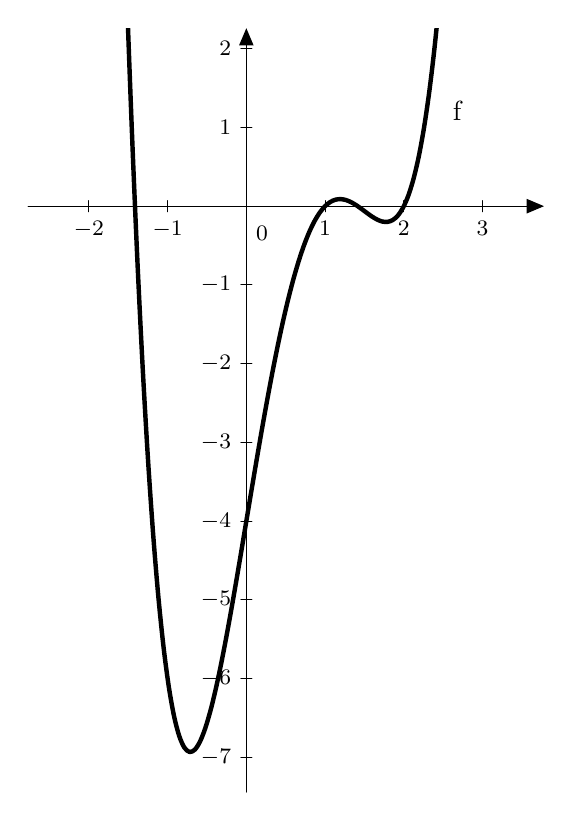
\begin{tikzpicture}[line cap=round,line join=round,>=triangle 45,x=1.0cm,y=1.0cm]
    \draw[->,color=black] (-2.77,0) -- (3.78,0);
    \foreach \x in {-2,-1,1,2,3}
    \draw[shift={(\x,0)},color=black] (0pt,2pt) -- (0pt,-2pt) node[below] {\footnotesize $\x$};
    \draw[->,color=black] (0,-7.44) -- (0,2.26);
    \foreach \y in {-7,-6,-5,-4,-3,-2,-1,1,2}
    \draw[shift={(0,\y)},color=black] (2pt,0pt) -- (-2pt,0pt) node[left] {\footnotesize $\y$};
    \draw[color=black] (0pt,-10pt) node[right] {\footnotesize $0$};
    \clip(-2.77,-7.44) rectangle (3.78,2.26);
    \draw[line width=1.6pt, smooth,samples=100,domain=-2.7709659189295555:3.7776369933097222] plot(\x,{(\x)^4-3*(\x)^3+6*(\x)-4});
    \draw (2.5,1.46) node[anchor=north west] {f};
    \end{tikzpicture}
  \end{center}
  \item $f(x)=x^5-x^4-13x^3+13x^2+36x-36$
  \begin{center}
    \definecolor{cqcqcq}{rgb}{0.75,0.75,0.75}
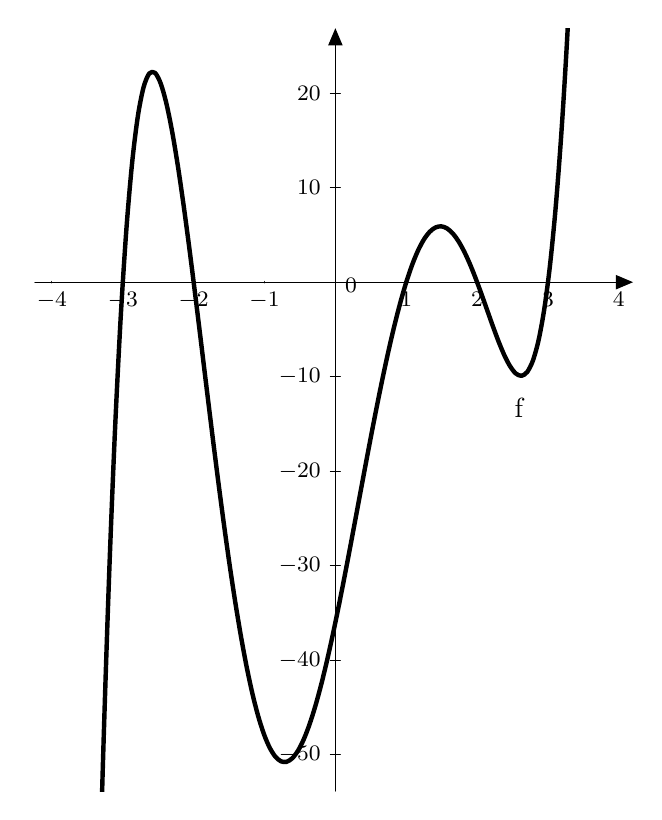
\begin{tikzpicture}[xscale=.9, yscale=.12, line cap=round,line join=round,>=triangle 45,x=1.0cm,y=1.0cm]
\draw[->,color=black] (-4.24,0) -- (4.2,0);
\foreach \x in {-4,-3,-2,-1,1,2,3,4}
\draw[shift={(\x,0)},color=black] (0pt,2pt) -- (0pt,-2pt) node[below] {\footnotesize $\x$};
\draw[->,color=black] (0,-53.86) -- (0,26.88);
\foreach \y in {-50,-40,-30,-20,-10,10,20}
\draw[shift={(0,\y)},color=black] (2pt,0pt) -- (-2pt,0pt) node[left] {\footnotesize $\y$};
\draw[color=black] (0pt,-10pt) node[right] {\footnotesize $0$};
\clip(-4.24,-53.86) rectangle (4.2,26.88);
\draw[line width=1.6pt, smooth,samples=100,domain=-4:4] plot(\x,{(\x)^5-(\x)^4-13*(\x)^3+13*(\x)^2+36*(\x)-36});
\draw (2.39,-11.21) node[anchor=north west] {f};
\end{tikzpicture}
  \end{center}
  \item $f(x)=x^4-\dfrac{23}{12}x^3+\dfrac{29}{24}x^2-\dfrac{1}{4}x$
  \begin{center}
    \definecolor{cqcqcq}{rgb}{0.75,0.75,0.75}
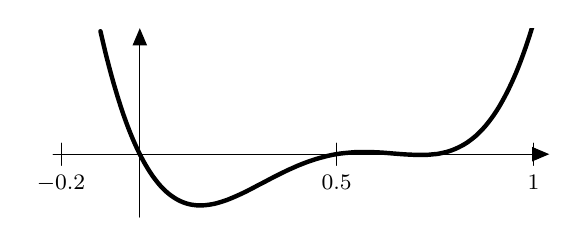
\begin{tikzpicture}[xscale=5, yscale=40,line cap=round,line join=round,>=triangle 45,x=1.0cm,y=1.0cm]
\draw[->,color=black] (-0.22,0) -- (1.04,0);
\foreach \x in {-0.2,0.5,1}
\draw[shift={(\x,0)},color=black] (0pt,.1pt) -- (0pt,-.1pt) node[below] {\footnotesize $\x$};
\draw[->,color=black] (0,-0.02) -- (0,0.04);
\foreach \y in {}
\draw[shift={(0,\y)},color=black] (2pt,0pt) -- (-2pt,0pt) node[left] {\footnotesize $\y$};
\clip(-0.22,-0.02) rectangle (1.04,0.04);
\draw[line width=1.6pt, smooth,samples=100,domain=-0.1:1] plot(\x,{(\x)^4-23/12*(\x)^3+29/24*(\x)^2-1/4*(\x)});
\draw (2.39,-12.67) node[anchor=north west] {f};
\end{tikzpicture}
  \end{center}
  \item $f(x)=x^5-15x^3+10x^2+60x-72$
  \begin{center}
    \definecolor{cqcqcq}{rgb}{0.75,0.75,0.75}
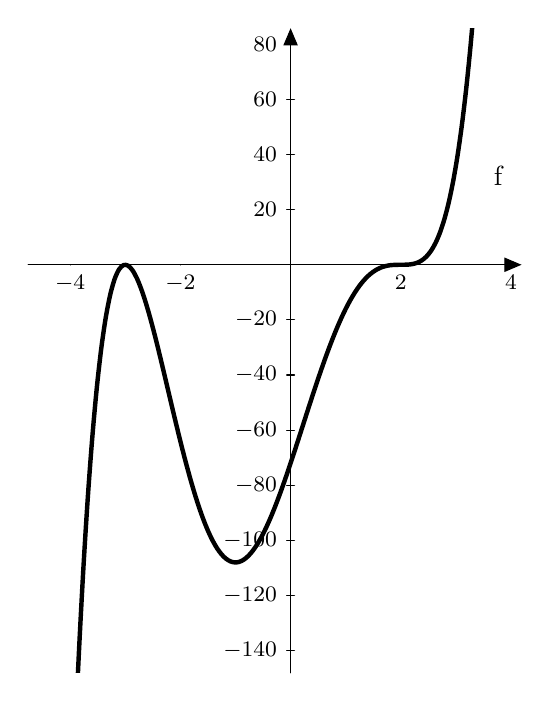
\begin{tikzpicture}[xscale=.7, yscale=.035,line cap=round,line join=round,>=triangle 45,x=1.0cm,y=1.0cm]
\draw[->,color=black] (-4.76,0) -- (4.19,0);
\foreach \x in {-4,-2,2,4}
\draw[shift={(\x,0)},color=black] (0pt,2pt) -- (0pt,-2pt) node[below] {\footnotesize $\x$};
\draw[->,color=black] (0,-148.05) -- (0,85.82);
\foreach \y in {-140,-120,-100,-80,-60,-40,-20,20,40,60,80}
\draw[shift={(0,\y)},color=black] (2pt,0pt) -- (-2pt,0pt) node[left] {\footnotesize $\y$};
\clip(-4.76,-148.05) rectangle (4.19,85.82);
\draw[line width=1.6pt, smooth,samples=100,domain=-4:4] plot(\x,{(\x)^5-15*(\x)^3+10*(\x)^2+60*(\x)-72});
\draw (3.51,39.24) node[anchor=north west] {f};
\end{tikzpicture}
  \end{center}
  \item $f(x)=x^6+2x^5-11x^4-12x^3+36x^2$
  \begin{center}
    \definecolor{cqcqcq}{rgb}{0.75,0.75,0.75}
    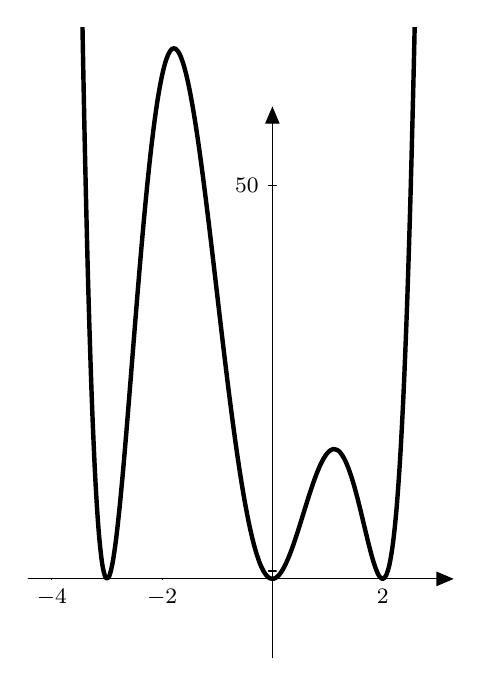
\begin{tikzpicture}[xscale=.7, yscale=.1, line cap=round,line join=round,>=triangle 45,x=1.0cm,y=1.0cm]
    \draw[->,color=black] (-4.43,0) -- (3.29,0);
    \foreach \x in {-4,-2,2}
    \draw[shift={(\x,0)},color=black] (0pt,2pt) -- (0pt,-2pt) node[below] {\footnotesize $\x$};
    \draw[->,color=black] (0,-10) -- (0,60);
    \foreach \y in {,50}
    \draw[shift={(0,\y)},color=black] (2pt,0pt) -- (-2pt,0pt) node[left] {\footnotesize $\y$};
    \clip(-4.43,-10) rectangle (3.29,70);
    \draw[line width=1.6pt, smooth,samples=100,domain=-3.6:2.7] plot(\x,{(\x)^6+2*(\x)^5-11*(\x)^4-12*(\x)^3+36*(\x)^2});
    \draw (-1.44,82.3) node[anchor=north west] {f};
    \end{tikzpicture}
  \end{center}
\end{enumerate}
\end{multicols}
\end{oefening}

\begin{oefening}
Bespreek door gebruik te maken van ICT (domein, bereik, nulwaarden, tekenverloop, stijgen\&dalen):
\begin{enumerate}[(a)]
  \itemsep0.5em
  \item $f(x)=(x-2)^2(x+4)^2$
  \item $f(x)=(x-16)^2-x^2-8x^4-64$
  \item $f(x)=x(x-1)(x-2)(x-3)(x-4)$
  \item $f(x)=-\dfrac{1}{8}(x^4+x^3-14x^2-8x+48)$
\end{enumerate}
\end{oefening}

\begin{oefening}
Beschouw de functie $f(x)=-\dfrac{1}{4}(x^4+3x^3-3x^2-9x)$, met als grafiek:
\begin{center}
\definecolor{cqcqcq}{rgb}{0.75,0.75,0.75}
\begin{tikzpicture}[line cap=round,line join=round,>=triangle 45,x=1.0cm,y=1.0cm]
\draw [color=cqcqcq,dash pattern=on 1pt off 1pt, xstep=1.0cm,ystep=1.0cm] (-4.31,-1.55) grid (3.31,2.64);
\draw[->,color=black] (-4.31,0) -- (3.31,0);
\foreach \x in {-4,-3,-2,-1,1,2,3}
\draw[shift={(\x,0)},color=black] (0pt,2pt) -- (0pt,-2pt) node[below] {\footnotesize $\x$};
\draw[->,color=black] (0,-1.55) -- (0,2.64);
\foreach \y in {-1,1,2}
\draw[shift={(0,\y)},color=black] (2pt,0pt) -- (-2pt,0pt) node[left] {\footnotesize $\y$};
\draw[color=black] (0pt,-10pt) node[right] {\footnotesize $0$};
\clip(-4.31,-1.55) rectangle (3.31,2.64);
\draw[line width=1.6pt, smooth,samples=100,domain=-4.306720586404644:3.3067938031642226] plot(\x,{(-1)/4*((\x)^4+3*(\x)^3-3*(\x)^2-9*(\x))});
\draw (1.54,2.02) node[anchor=north west] {f};
\end{tikzpicture}
\end{center}
Bespreek (domein, bereik, nulwaarden, tekenverloop, stijgen\&dalen).
\end{oefening}

\begin{oefening}
Construeer een veeltermfunctie van de vierde graad met nulwaarden $x_0=-4$, $x_1=2$ en $x_2=3$. De nulwaarde $x_1$ komt tweemaal voor (we zeggen dat deze multipliciteit 2 heeft). De functie moet negatief zijn voor $x\in]-\infty,-4[$.
\end{oefening}



\newpage
\section{Veeltermongelijkheden}


\subsection{Eerstegraadsveeltermongelijkheden}


\begin{oefening}
Los op in $\mathbb{R}$:
\begin{multicols}{2}
\begin{enumerate}[(a)]
  \itemsep0.6em
  \item $x-5<0$
  \item $2x+3\geq 2$
  \item $8x-3<0$
  \item $7\leq 7-49x$
\end{enumerate}
\end{multicols}
\end{oefening}


\subsection{Tweedegraadsveeltermongelijkheden}


\begin{oefening}
Los op in $\mathbb{R}$:
\begin{multicols}{2}
\begin{enumerate}[(a)]
  \itemsep0.6em
  \item $-6x^2+13x-6\leq 0$
  \item $80x^2-20x-10\geq 0$
  \item $-15x^2+30x+45\geq 45$
  \item $x^2+4x+4 < 0$
  \item $(x+2)^2 > 4x$
  \item $-x^2 > -4x$
\end{enumerate}
\end{multicols}
\end{oefening}



\subsection{Veeltermongelijkheden van hogere graad oplossen}


\begin{oefening}
  Los op in $\mathbb{R}$:
  \begin{multicols}{2}
    \begin{enumerate}[(a)]
      \itemsep0.6em
    \item $x^2(2-x)\leq6-5x$
    \item $2x^3-x^2-13x<6$
    \item $x(x+2)^2\leq9+x-x^2$
    \item $x(x^2+12)>2(3x^2+4)$
    \item $x(x^2-3)<2$
    \item $x^4+27x^2+4x<36+12x^3$
    \item $12+x^3\geq13x$
    \item $x^4-71x^2-66x-4x^3>0$
    \item $2x(x+1)-\frac{1}{2}x<2(x+1)^2$
    \item $(1+2x)^2\leq(x-2)(x+2)$
    \item $x(x+1)-\frac{x+3}{10}$
    \item $-x^3+2x^2\leq6-5x$
    \item $\frac{x(x^2-3)}{2}<1$
    \item $x^3\geq8$
    \end{enumerate}
  \end{multicols}
\end{oefening}

\begin{oefening}
  Welke reële getallen zijn groter dan hun derdemacht?
\end{oefening}

\begin{oefening}
  Voor welke reële getallen is het kwadraat groter dan de derdemacht
\end{oefening}


\subsection{Veeltermongelijkheden oplossen m.b.v. Geogebra}

\begin{oefening}
  \begin{enumerate}[(a)]
  \item Bestaan er veeltermongelijkheden van de tweede graad die geen
    oplossingen hebben? Zo ja, geef een voorbeeld. Verklaar dit
    grafisch.
  \item Bestaan er veeltermongelijkheden van de derde graad die geen
    oplossingen hebben? Zo ja, geef een voorbeeld. Verklaar dit
    grafisch.
  \end{enumerate}
\end{oefening}


\newpage
\section{Toepassingen}

\begin{oefening}
Kasper heeft na zijn verjaardagsfeest nog een vuurpijl over. Hij vuurt die af vanuit zijn slaapkamer. De pijl vliegt eerst lichtjes naar beneden, maar gaat uiteindelijk toch de lucht in om na 5 seconden te ontploffen. De hoogte $h$ (in meters) in functie van de tijd $x$ (in seconden) wordt beschreven door de formule:
$$h=x^3-4x^2+2x+8$$
\begin{enumerate}[(a)]
  \item Hoe hoog is de slaapkamer van Kasper?
  \item Hoe hoog is de vuurpijl na 5 seconden?
  \item Wanneer vliegt de vuurpijl op een hoogte van 5 meter?
\end{enumerate}
\end{oefening}

\begin{oefening}
De hoogte $h$ (in meters) van een luchtballon $t$ uren na het opstijgen wordt gegeven door de functie:
$$h(t)=-t^4+9t^3-120t^2+500t$$.
\begin{enumerate}[(a)]
  \item Bereken na hoeveel tijd de ballon weer op de grond komt.
  \item Na hoeveel uren vliegt de ballon op een hoogte van 400m?
\end{enumerate}
\end{oefening}

\begin{oefening}
Een bedrijf produceert fietscomputertjes. De bedrijfsleiding wil weten hoeveel computertjes per uur moeten geproduceerd worden om winst te maken in de huidige situatie. Het verband tussen de winst $W$ (in euro) en de productie $x$ (aantal geproduceerde computertjes) per uur is:
$$W(x)=-\dfrac{1}{2}x^3+8x^2-\dfrac{55}{2}x$$
\begin{enumerate}[(a)]
  \item Bij welke productie zal de winst 0 euro bedragen?
  \item Bij welke productie wordt er winst gemaakt?
  \item Bij welke productie wordt er verlies gemaakt?
  \item Bij welke productie is de winst gelijk aan 36 euro?
\end{enumerate}
\end{oefening}

\begin{oefening}
Een game studio modelleert de winst op zijn laatste computer spelletje met behulp van
$$W(n)=-2n^2+28n-90$$ waarbij $n$ het aantal per honderdduizend verkochte spelletjes is en waarbij $W$ de winst is in miljoenen euro.
\begin{enumerate}[(a)]
  \item Hoeveel spelletjes moet het bedrijf op zijn minst verkopen om uit de kosten te geraken?
  \item Wanneer maakt het bedrijf winst/verlies?
\end{enumerate}
\end{oefening}

\begin{oefening}
De bevolking van een Limburgse gemeente is sinds 1980 geëvolueert volgens de functie $$f(x)=5x^3-85x^2+80x+4000$$ waarbij $x=0$ overeenkomt met het jaar 1980.
\begin{enumerate}[(a)]
  \item Hoeveel inwonders waren er in 1980?
  \item In welk jaar zullen er 31000 inwoners zijn? (één tijdstip volstaat)
\end{enumerate}
\end{oefening}

\begin{oefening}
Een groep bergbeklimmers vertrekt op tocht.  De route die zij volgen wordt beschreven	door de volgende veeltermfunctie $$h(x)=90x^2-10x^3$$ met
\begin{itemize}
  \item h = hoogte in meter
  \item x = tijd in uren ( x = 0 is het tijdstip waarop de groep begint met de beklimming)
\end{itemize}
\begin{enumerate}[(a)]
  \item Hoelang duurt de tocht?
  \item Na hoeveel uur bereikt de groep een hoogte van 800 meter? (één tijdstip volstaat)
\end{enumerate}
\end{oefening}

\begin{oefening}
Een bedrijf produceert gps-toestellen voor auto’s.  De bedrijfsleiding wil weten hoeveel toestellen er per uur geproduceerd moeten worden om winst te maken in de huidige situatie.  Het verband tussen de winst $W$ (in euro) en de productie $x$ (aantal geproduceerde toestellen) per uur is
$$W=-\dfrac{3}{2}x^3+24x^2-72x\;.$$
\begin{enumerate}[(a)]
  \item Bij welke productie is de winst gelijk aan 0 euro ($W = 0$)?
  \item Bij welke productie wordt er winst ($W > 0$) en bij welke productie wordt er verlies ($W < 0$) gemaakt?
  \item Bij welke productie is de winst gelijk aan 108 euro?  (één oplossing volstaat)
\end{enumerate}
\end{oefening}

\begin{oefening}
Ibuprofen is een pijnstillend middel.  Om het aantal mg $m$ van het middel in de bloedsomloop te schatten, $t$ uren nadat 100 mg van dit middel werd ingenomen, gebruiken we het verband
$$m(t)=-t^4+4t^3-9t^2+36t$$
met $m =$ aantal $\mg$ van het middel Ibuprofen in het bloed $t = $ aantal uren nadat je $100 \mg$ Ibuprofen hebt ingenomen.
\begin{enumerate}[(a)]
  \item Wanneer is het pijnstillend middel uitgewerkt?
  \item Op welk tijdstip is het opgenomen gehalte in het bloed gelijk aan $30 \mg$? (één tijdstip volstaat)
\end{enumerate}
\end{oefening}

\begin{oefening}
Het aantal bezoekers dat zich op een zonnige dag in de maand juli in een dierenpark bevindt, zou je kunnen benaderen door het functievoorschrift
$$n(t)=100t+140t^2-15t^3$$
met $n(t)$ het aantal bezoekers op tijdstip $t$ in uren, waarbij $t=0$ overeenkomt met 9u 's morgens (het openingsuur van het dierenpark).
\begin{enumerate}[(a)]
  \item Bepaal het sluitingsuur van het dierenpark.
  \item Hoeveel bezoekers waren er om 12 uur 's middags?
\end{enumerate}
\end{oefening}

\begin{oefening}
Stef woont in een appartement en laat van in zijn venster een opgeblazen ballon vliegen.  Deze gaat eerst naar beneden om dan snel de hoogte in te gaan.  De baan kan beschreven worden door de volgende veeltermfunctie
$$h(x)=-4x^3+16x^2-6x+12\;.$$
Hierbij is
\begin{itemize}
  \item $h$ de hoogte in meter,
  \item $x$ de afstand in meter.
\end{itemize}
Hoe hoog is de vensterbank van het raam waaruit Stef de ballon laat vliegen? Duid het juiste antwoord aan en leg uit waarom je die oplossing hebt gekozen.\\
\begin{center}
  \begin{tabular}{|ccccc|}
  \hline
  4 meter & 6 meter & 8 meter & 12 meter & 18 meter\\[0.2cm]
  \hline    
  \end{tabular}
\end{center}
\end{oefening}

\begin{oefening}{\scriptsize\em Opmerking: Deze oefening kon je vorig jaar ook al oplossen want het betreft een tweedegraadsveeltermfunctie}\\
Een ecologische verbindingsbrug moet worden ontworpen over een belangrijke snelweg. De brug over de snelweg wordt gebouwd in de vorm van een parabool. De snelweg is 8 meter breed en wordt gecentreerd onder de parabolische boog. De brug moet in het totaal een breedte van $16 \m$ overspannen. De brug moet een minimale hoogte van 4 m over de snelweg te bieden.
\begin{enumerate}[(a)]
  \item Teken de parabool en de snelweg, label alle relevante afmetingen.
  \item Plaats een coördinatenstelsel op de tekening zodat de $y$-as de snelweg in het midden doorsnijdt en de $x$-as gelegen is aan de voet van de brug.
  \item Vind de kwadratische functie in standaardvorm die de hoogte van de brug $y$ geeft als functie van de horizontale afstand van het centrum $x$.
  \item Bepaal de maximale hoogte van de boog over de snelweg.
\end{enumerate}
\end{oefening}



\end{document}
